\documentclass[a4paper,10pt,twoside]{article}

\usepackage[top=1in, bottom=1in, left=1in, right=1in]{geometry}
\usepackage[utf8]{inputenc}
%\usepackage[spanish,es-ucroman,es-noquoting]{babel}
\usepackage{fancyhdr}
\usepackage{lastpage}
\usepackage{graphicx}



%%%%%%%%%% Configuración de Fancyhdr - Inicio %%%%%%%%%%
\pagestyle{fancy}
\thispagestyle{fancy}
\lhead{TP1, Sistemas Operativos}
\renewcommand{\footrulewidth}{0.4pt}
\cfoot{\thepage /\pageref{LastPage}}

\fancypagestyle{caratula} {
   \fancyhf{}
   \cfoot{\thepage /\pageref{LastPage}}
   \renewcommand{\headrulewidth}{0pt}
   \renewcommand{\footrulewidth}{0pt}
}

%%%%%%%%%% Macros de tikz - Fin %%%%%%%%%%


\begin{document}


%%%%%%%%%%%%%%%%%%%%%%%%%%%%%%%%%%%%%%%%%%%%%%%%%%%%%%%%%%%%%%%%%%%%%%%%%%%%%%%
%% Carátula                                                                  %%
%%%%%%%%%%%%%%%%%%%%%%%%%%%%%%%%%%%%%%%%%%%%%%%%%%%%%%%%%%%%%%%%%%%%%%%%%%%%%%%


\thispagestyle{caratula}

\begin{center}


\includegraphics[height=2cm]{DC.png} 
\hfill

\includegraphics[height=2cm]{UBA.jpg} 

\vspace{2cm}

Departamento de Computación,\\
Facultad de Ciencias Exactas y Naturales,\\
Universidad de Buenos Aires

\vspace{4cm}

\begin{Huge}
TP1 - Scheduling
\end{Huge}

\vspace{0.5cm}

\begin{Large}
Sistemas Operativos
\end{Large}

\vspace{1cm}

Segundo Cuatrimestre de 2014

\vspace{4cm}

\vspace{0.5cm}

\begin{tabular}{|c|c|c|}
\hline
Apellido y Nombre & LU & E-mail\\
\hline
Cisneros Rodrigo		& 920/10 & rodricis@hotmail.com\\
Rodr\'iguez, Agust\'in	& 120/10 & agustinrodriguez90@hotmail.com\\
Tripodi, Guido			& 843/10 & guido.tripodi@hotmail.com\\
\hline
\end{tabular}

\end{center}

\newpage


%%%%%%%%%%%%%%%%%%%%%%%%%%%%%%%%%%%%%%%%%%%%%%%%%%%%%%%%%%%%%%%%%%%%%%%%%%%%%%%
%% Índice                                                                    %%
%%%%%%%%%%%%%%%%%%%%%%%%%%%%%%%%%%%%%%%%%%%%%%%%%%%%%%%%%%%%%%%%%%%%%%%%%%%%%%%


\tableofcontents

\newpage


%%%%%%%%%%%%%%%%%%%%%%%%%%%%%%%%%%%%%%%%%%%%%%%%%%%%%%%%%%%%%%%%%%%%%%%%%%%%%%%
%% Introducción                                                              %%
%%%%%%%%%%%%%%%%%%%%%%%%%%%%%%%%%%%%%%%%%%%%%%%%%%%%%%%%%%%%%%%%%%%%%%%%%%%%%%%


\section{Introducción}

\indent \indent En este Trabajo Práctico estudiaremos diversas implementaciones de algoritmos de scheduling. 
Haciendo uso de un simulador provisto por la cátedra podremos reprensentar el comportamiento de estos algoritmos. 
Implementaremos dos Round-Robin, uno que permite migración de tareas entre núcleos y otro que no y a través de experimentación intentaremos comparar ambos algoritmos. 
Asimismo, basándonos en un paper implementaremos una versión del algoritmo $Lotery$ y 
mediante experimentos intentaremos comprobar ciertas propiedades que cumple el algoritmo.\\

%%%%%%%%%%%%%%%%%%%%%%%%%%%%%%%%%%%%%%%%%%%%%%%%%%%%%%%%%%%%%%%%%%%%%%%%%%%%%%%
%% Desarrollo                                                                %%
%%%%%%%%%%%%%%%%%%%%%%%%%%%%%%%%%%%%%%%%%%%%%%%%%%%%%%%%%%%%%%%%%%%%%%%%%%%%%%%

\newpage
\section{Desarrollo y Resultados}

\section{Parte I – Entendiendo el simulador simusched}


\subsection{Ejercicios}
\begin{itemize}
 \item \textbf{Ejercicio 1 }
 En primer lugar, deberán implementar un Read-Write Lock libre de inanición utilizando únicamente Variables de Condición POSIX 
 y  respetando la interfaz provista en los archivos backend-multi/RWLock.h y backend-multi/RWLock.cpp
\end{itemize}

\subsection{Resultados y Conclusiones}

\subsubsection[Resolución Ejercicio 1]{Ejercicio 1}

\indent Nuestra implementación del Read-Write Lock se bas\'{o} en el pseudoc\'{o}digo implementado en el libro $The$ $Little$ $Book$ $of$ $Semaphores$
al resolver la inanición producida en el problema de $Readers-writers$.\\

Se utilizaron 3 Semaphores, los cuales son:\\
\begin{itemize}
 \item roomEmpty
 \item turnstile
 \item readers$\_$mutex
\end{itemize}

Y ademas, un entero denominado $readers$\\

Comenzando por la implementación de los lectores, el pseudoc\'{o}odigo del libro mencionado es el siguiente:\\

\begin{verbatim}
            turnstile.wait()
            turnstile.signal()

            readSwitch.lock(roomEmpty)
                # critical section for readers
            readSwitch.unlock(roomEmpty)
\end{verbatim}

De aquí nuestro código implementado fue el siguiente:\\

\begin{center}
            \textbf{READERS LOCK}     
\end{center}

 
\begin{verbatim}
            pthread_mutex_lock(&turnstile);
            pthread_mutex_unlock(&turnstile);

            pthread_mutex_lock(&readers_mutex);
            readers++;
            pthread_mutex_unlock(&readers_mutex);
\end{verbatim}

Como se puede observar en el c\'{o}digo del lock del read, el lector realiza un lock (wait) y unlock (signal) del Semaphores $turnstile$
para tener su turno y que ningún otro lo saque.\\
Por consiguiente, se realiza el lock del mutex que se encuentra vinculado al entero $readers$, ya que este
aumentará su cantidad en 1 para que, de esta manera nadie pueda modificarlo, y luego es liberado dicho mutex ($readers\_mutex$).\\

Luego, nuestro $READ$ $UNLOCK$ fue el siguiente:\\

\begin{center}
            \textbf{READERS UNLOCK}
\end{center}

 
\begin{verbatim}
            pthread_mutex_lock(&readers_mutex);
            readers--;
            if (readers == 0) {
                pthread_cond_signal(&room_empty);		
            }
            pthread_mutex_unlock(&readers_mutex);
\end{verbatim}

En esta implementación, primero se realiza un lock del Semaphore vinculado al entero $readers$ ya que este disminuirá en 1.\\
Luego, se realiza una consulta chequeando el valor del entero, si este es 0 se le dara un signal a la variable de condici\'{o}n
$room\_empty$ para notificarle al escritor que ya no queda ning\'{u}n lector y puede proceder a escribir.\\
Por último, se libera el mutex $readers\_mutex$.\\

Continuando con el escritor, el pseudoc\'{o}digo fue el siguiente:\\

\begin{verbatim}

            turnstile.wait()
            roomEmpty.wait()
                # critical section for writers
            turnstile.signal()

            roomEmpty.signal()

\end{verbatim}

De aquí, nuestra implementación final fue:\\

\begin{center}
            \textbf{WRITERS LOCK}
\end{center}

 
\begin{verbatim}
            pthread_mutex_lock(&turnstile);
            pthread_mutex_lock(&readers_mutex);
            while(readers != 0)
                  pthread_cond_wait(&room_empty, &readers_mutex);
            pthread_mutex_unlock(&readers_mutex);
\end{verbatim}

Inicialmente en nuestra implementación del WRITE LOCK, se realiza un lock del Semaphore $turnstile$ para que nadie pueda quitarle el turno, se realiza un
lock del mutex vinculado al entero, y luego se ingresa a un ciclo siempre que $readers$ sea distinto de 0, esto se realiza
para luego poder ejecutar la funcion $pthread\_cond\_wait$ para que esta misma tenga un funcionamiento correcto y seguro al
chequear la condición sobre $room\_empty$.\\
Una vez que se salga del ciclo o no se ingrese al mismo se libera el mutex $readers\_mutex$.\\

Luego, la implementación del unlock fue:\\
\begin{center}
           \textbf{WRITERS UNLOCK}
\end{center}

 
\begin{verbatim}
           pthread_mutex_unlock(&turnstile);
\end{verbatim}

Para la implementación del unlock del writer solo se libera el Semaphore $turnstile$.\\

De esta manera, con dicha implementación, siempre que llegue un escritor el mismo tendrá su turno sin producirse inanición.
Ya que, en caso de haber lectores y llegar un escritor, estos terminar\'{a}n de leer y en caso 
de llegar nuevos lectores deberán esperar a que el escritor finalice su ejecución.\\

\newpage
%\subsection{Filtro Miniature}

\section{Parte II: Extendiendo el simulador con nuevos schedulers}


\subsection{Ejercicios}
\begin{itemize}
 \item 
\textbf{Ejercicio 4}  Completar la implementación del scheduler Round-Robin implementando los
metodos de la clase SchedRR en los archivos sched rr.cpp y sched rr.h. La implementacion
recibe como primer parametro la cantidad de nucleos y a continuacion los valores de sus
respectivos quantums. Debe utilizar una unica cola global, permitiendo ası la migracion de
procesos entre nucleos.
\item \textbf{Ejercicio 5}Disene un lote con 3 tareas de tipo TaskCPU de 50 ciclos y 2 de tipo TaskConsola
con 5 llamadas bloqueantes de 3 ciclos de duracion cada una. Ejecutar y graficar la simulacion
utilizando el scheduler Round-Robin con quantum 2, 10 y 50.\\
Con un cambio de contexto de 2 ciclos y un solo nucleo calcular la latencia, el waiting
time y el tiempo total de ejecucion de las cinco tareas para cada quantum. 
¿En cual es mejor cada uno? ¿Por que ocurre esto?
\item \textbf{Ejercicio 6} Grafique el mismo lote de tareas del ejercicio anterior para el scheduler FCFS.
Haciendo referencia a lo que se observa en los graficos de este ejercicio y el anterior, explique
las diferencias entre un scheduler Round-Robin y un FCFS.
\item \textbf{Ejercicio 7} Grafique el mismo lote de tareas del ejercicio anterior para el scheduler FCFS.
Haciendo referencia a lo que se observa en los graficos de este ejercicio y el anterior, explique
las diferencias entre un scheduler Round-Robin y un FCFS.
\item \textbf{Ejercicio 8} Implemente un scheduler Round-Robin que no permita la migracion de procesos
entre nucleos (SchedRR2). La asignación de CPU se debe realizar en el momento en que se produce la carga 
de un proceso (load). El nucleo correspondiente a un nuevo proceso sera aquel
con menor cantidad de procesos activos totales (RUNNING + BLOCKED + READY).Explique un escenario real 
donde la migracion de nucleos sea beneficiosa y uno donde no (mencione
especificamente que metricas de comparacion vistas en la materia mejorarıan en cada caso).
Disene un lote de tareas en nuestro simulador que represente a cada uno de esos escenarios
y grafique su resultado para cada implementacion. Calcule y compare en cada grafico las
metrica que menciono.

\end{itemize}


\subsection{Resultados y Conclusiones}

\subsubsection[Resolución Ejercicio 4]{Ejercicio 4}
Para desarrollar la implementación del scheduler $Round-Robin$ y que este funcione de una forma correcta
utilizamos una serie de estructuras puntuales. \\
Las mismas son las siguientes:\\
\begin{enumerate}
 \item Una cola global, la cual nombramos $q$, esta contiene los $PID$ de los procesos activos que no estan
 bloqueados y en el tope de la misma se encuentra el próximo proceso a correr. Esta cola,
 fue desarrollada para que cuando se desaloje un proceso por finalizar su $quantum$ la misma pase al final de
 la cola y generando el ciclo acorde al comportamiento de este scheduler.
 \item Un vector denominado $cores$, este tiene en su elemento $i$ el pid correspondiente a
al proceso que está corriendo en el core $i+1$. Inicializamos todos los elementos en -1, esto
corresponde a la Idle Task, de esta forma reconocemos que no se cargaron procesos en los núcleos.
\item Un vector $quantum$ guarda en la posicion $i$ el quantum que se dispuso a cada núcleo.
\item Un vector $quantumActual$ aqui guardaremos la cantidad de ticks que le quedan al proceso
desde que fue cargado en el core.
\item Una lista de $bloqueados$ esta tendra procesos que se bloquearon cuando estaban corriendo.
\end{enumerate}

De esta manera, con estas estructuras nos permiten determinar para cada tarea, cuándo, y cuánto 
de su quantum consumieron de forma que podamos desalojarla correctamente.\\

A su vez, tomamos ciertas decisiones en esta implementación:
\begin{itemize}
 \item Si una tarea se encuentra bloqueada cuando se produce el tick del reloj, esta misma es desalojada
de la cola global, y agregada en un lista de bloqueados. Además, sera reseteado el quantum, se le
dará inicio a la próxima tarea que se encuentre ready y cuando el sistema operativo, nos envie una
señal de unblock, la tarea desalojada regresará al final de la cola global.

\end{itemize}


\subsubsection[Resolución Ejercicio 5]{Ejercicio 5}

EN ESTE PUNTO SIRVE TODO LO ESCRITO SOLO HAY Q CAMBIAR GRAFICOS!

\indent El algoritmo de scheduler \textbf{Round-Robin} tiene como caracter\'istica asignar a todas las tareas 
un determinado tiempo m\'aximo de procesamiento, a esto se lo llama $quantum$. \\
\indent Este tiempo esta definido para cada n\'ucleo en particular, dependiendo de en cu\'al de ellos est\'en 
ejecutando los procesos, se les asignar\'a el respectivo tiempo m\'aximo.\\
\indent Otra caracter\'istica del \textbf{Round-Robin} es que las tareas se encolan y se ejecutan c\'iclicamente. 
Osea que cuando se deja de ejecutar, si no termin\'o su ejecuci\'on, la tarea se encolar\'a al final de la lista. 
Como elecci\'on de diseño, elegimos que se use una cola global para todos los procesadores, aunque tambi\'en
se podr\'ia tener una cola para cada n\'ucleo. \\
\indent A su vez, tambi\'en puede ocurrir una tarea no consuma todo su $quantum$. 
Ya sea porque la tarea se bloquea (haciendo uso de dispositivos de entrada/salida) o porque termine su ejecuci\'on.\\
\indent En caso de haber terminado, nuestro algoritmo pone a correr directamente la pr\'oxima tarea de acuerdo al orden 
circular que se estableci\'o y la tarea que finaliz\'o se desalojar\'a por completo y no sera considerada nuevamente. \\
\indent En caso de haberse bloqueado, esta misma dejar\'a de ser considerada hasta que se desbloquee, 
perdiendo el quantum que le quedaba si hubiere. 
Autom\'aticamente, seguir\'a corriendo la pr\'oxima tarea que se encuentre en la cola global. 
Cuando el proceso se desbloquee, ser\'a encolada nuevamente al final de dicha cola.   \\

\indent Para corroborar que el comportamiento era el deseado, nos solicitaron 1 lotes de tareas compuestos por tareas
del tipo $taskConsola$ y $taskCpu$, trabajando con 1 cores y utilizando distintos $quantum$ para cada uno de los mismos.\\

El lote de tareas fue el siguiente:
\begin{verbatim}
                                   *3 TaskCPU 50
                                   *2 TaskConsola 5 3 3
\end{verbatim}

Obteniendo los siguientes resultados:

\begin{center}

    
	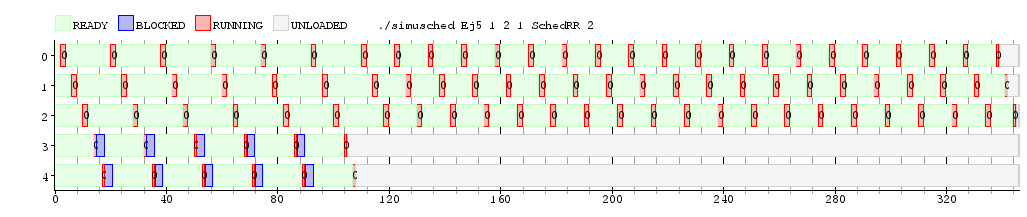
\includegraphics[width=450pt]{./Test/ej5_2.png}
	{$Lote 1$ - Scheduler RR - 1 core - 2 quantum}	
 
\end{center}

\begin{center}
  	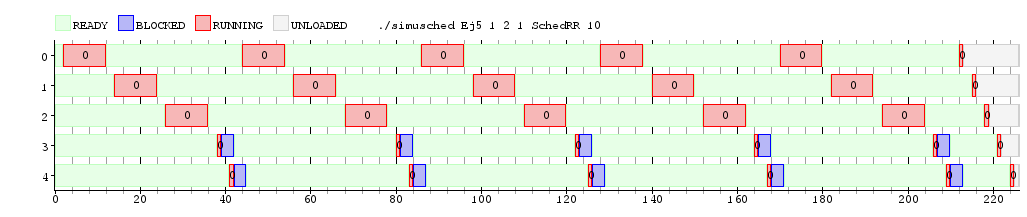
\includegraphics[width=450pt]{./Test/ej5_10.png}
	  {$Lote 1$ - Scheduler RR - 1 core - 10 quantum}	
\end{center}

\begin{center}
  	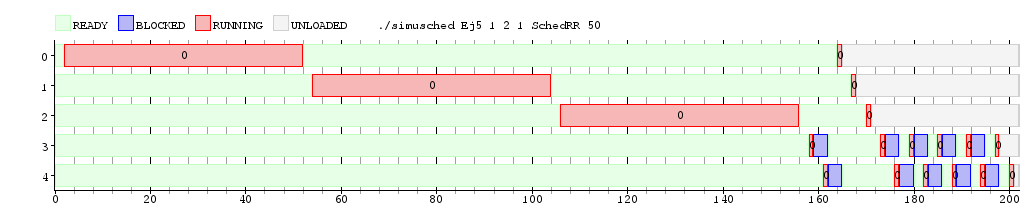
\includegraphics[width=450pt]{./Test/ej5_50.png}
	  {$Lote 1$ - Scheduler RR - 1 core - 50 quantum}	
\end{center}

\indent Se puede observar el cambio de tareas cíclico tanto porque terminaron su quantum o porque se bloquearon.\\


\indent Luego de estos experimentos pudimos observar ciertos puntos del comportamiento del Round-Robin:\\
\begin{itemize}
\item  Carácter circular del algoritmo.
\item  Desalojo de las tareas cuando se bloquean o terminan y la inmediata asignación del núcleo a la siguiente tarea en caso de existir alguna.
\item  Libre de inanición.
\item  Una tarea bloqueada es ignorada por el scheduler hasta que se desbloquee.
\end{itemize}

\indent Finalmente, dado su carácter circular y equitativo, podemos afirmar que todas las tareas que 
estén en condiciones de correr serán ejecutadas y ninguna será negada de tiempo de procesamiento.\\


\subsubsection[Resolución Ejercicio 5]{Ejercicio 6}

El lote de tareas solicitado fue el siguiente:
\begin{verbatim}
                                   *3 TaskCPU 50
                                   *2 TaskConsola 5 3 3
\end{verbatim}

Obteniendo los siguientes resultados:

\begin{center}
  	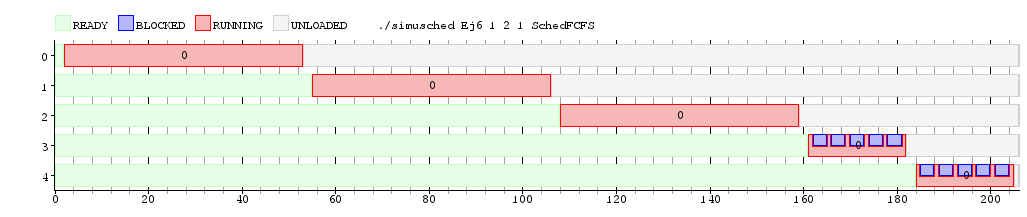
\includegraphics[width=450pt]{./Test/ej6.png}
	  {$Lote 1$ - Scheduler FCFS - 1 core}	
\end{center}

\indent A modo de analisis, hemos obtenido las siguientes conclusiones:\\

\begin{itemize}
 \item 
\end{itemize}


\subsubsection[Resolución Ejercicio 5]{Ejercicio 7}

\subsubsection[Resolución Ejercicio 8]{Ejercicio 8}

EN ESTE SOLO FALTARIA DECIR EL CASO REAL TRATANDO DE USAR NUESTRO LOTE YA HECHO

La idea principal de esta nueva versión de $Round-Robin$ se centraliza en que no permita migración entre
cores, esto se basa principalmente en utilizar una cola para cada núcleo por separado, y en cada
cola respectiva se encolaran las tareas que fueron asignadas inicialmente a cada nucleo.\\
Para desarrollar este tipo de algoritmo, el cual denominaremos $RR2$, utilizamos estructuras
puntuales, enunciadas a continuación:\\
\begin{itemize}
 \item Un vector $quantum$ y otro $quantumActual$, los cuales siguen cumpliendo la misma funcion que
 en Round-Robin 1.
 \item Un vector de colas denominado $colas$, en el cual, en la posición $i$ encontraremos la cola correspondiente
 a ese núcleo de procesamiento.
 \item Un diccionario de $Bloqueados$, donde la clave contendra el número de core, y en definición
 la tareas bloqueadas de ese core. Esto nos beneficiara cuando haya que reubicarla en la cola de procesos ready.
 \item Un vector de enteros $cantidad$, que como la palabra lo define, tendrá en cada posición $i$ 
 la totalidad de las tareas, ya sea bloqueadas, activas o en estado ready que tiene asignado ese core, beneficiandonos
 la determinación del núcleo al que se le asignará la tarea al momento de cargarla.
\end{itemize}
Cuando se carga una tarea, previamente, se chequeará que core tiene menor cantidad de procesos totales asignados (
aqui es donde el vector $cantidad$ entra en juego). Una vez que se obtiene este nucleo, se agrega 
la tarea a la cola correspondiente y se actualiza la cantidad sumando una unidad.\\
\indent Al bloquearse un proceso, se define una nueva entrada en el diccionario $bloqueados$ con el
pid y el nucleo correspondiente. De esta forma, al desbloquearse, colocamos la tarea en la cola del core
correspondiente y eliminamos la entrada del diccionario. Así logramos resolver el inconveniente de la nula
migración entre nucleos.\\
\indent Finalmente, cuando una tarea finaliza, la quitamos y descontamos una unidad a la posición $i$ del vector
$cantidad$. Esta es la única vez, en la cual se descuenta. Aunque una tarea se bloquee, la misma
seguirá contando en el vector. De esta forma se cumplirá, que las tareas son asignadas a los cores
con menor cantidad de tareas.\\
Luego de realizar dicha implementación, en comparación al Round-Robin original, hemos conjeturado 
las siguientes hipótesis:

\begin{enumerate}
 \item Dados un mismo lote de tareas y una misma configuración del scheduler (mismos costo en cambio
de contexto y quantum) un único núcleo de procesamiento, ambos algoritmos deben comportarse
de la misma manera.
\item Comportamiento menos eficiente en el RR2 con respecto al paralelismo, ya que al no permitir
migración de nucleos este se pierde.
\item Comportamiento más eficiente en el RR2 con lotes de tareas que se bloquean un gran numero
de veces. Esto surge ya que el Round-Robin original, es mas proclive a realizar cambios de contexto con la posibilidad
de darse un cambio de core.
\end{enumerate}

Por consiguiente, procederemos a demostrar lo conjeturado.\\

Iniciando con nuestra primer conjetura:\\

\textbf{Dados un mismo lote de tareas y una misma configuración del scheduler 
 (mismos costo en cambio de contexto y quantum)
un único núcleo de procesamiento, ambos algoritmos deben comportarse
de la misma manera.}\\

Trabajando con el lote que mencionamos a continuación:
    
    \begin{verbatim}
                                     TaskCPU 70
                                     TaskConsola 2 4 5
                                     TaskCPU 40
                                     TaskConsola 3 2 3
                                     TaskCPU 30
    \end{verbatim}

Utilizando un $quantum$ igual a 5 y un cambio de contexto igual a 1 obtuvimos 
resultados muy marcados, viendose notoriamente lo que queremos demostrar.\\

\begin{center}
    	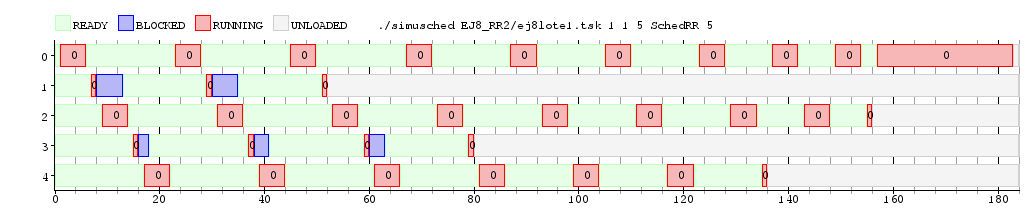
\includegraphics[width=450pt]{./EJ8_RR2/dif1corerr.png}
	{$Lote 1$ - Round Robin - 1 core - Quantum = 5 - cambio de contexto = 1}	
 \end{center}
 
 \begin{center}
    	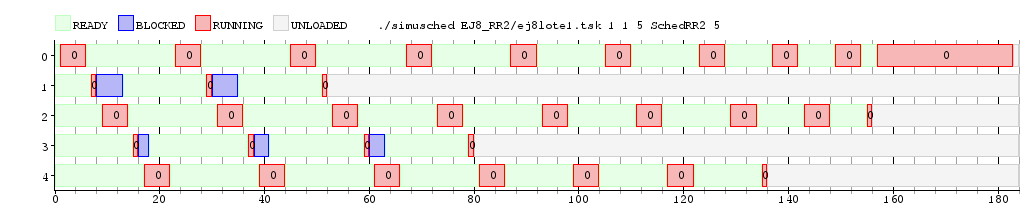
\includegraphics[width=450pt]{./EJ8_RR2/dif1corerr2.png}
	{$Lote 1$ - Round Robin 2 - 1 core - Quantum = 5 - cambio de contexto = 1}	
 \end{center}

Continuando con un lote distinto para ser mas precisos:

 \begin{verbatim}
                                     TaskCPU 70
                                     TaskConsola 5 6 7
                                     TaskCPU 40
                                     TaskConsola 10 9 8
                                     TaskCPU 30
 \end{verbatim}
 
Llegamos a lo siguiente:\\

 \begin{center}
    	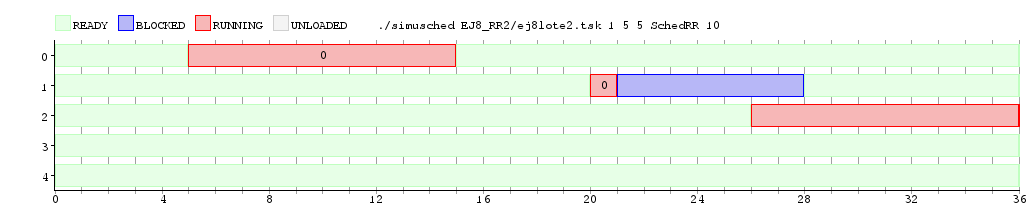
\includegraphics[width=450pt]{./EJ8_RR2/dif2corerr.png}
	{$Lote 2$ - Round Robin - 1 core - Quantum = 10 - cambio de contexto = 5}	
 \end{center}
 
 \begin{center}
    	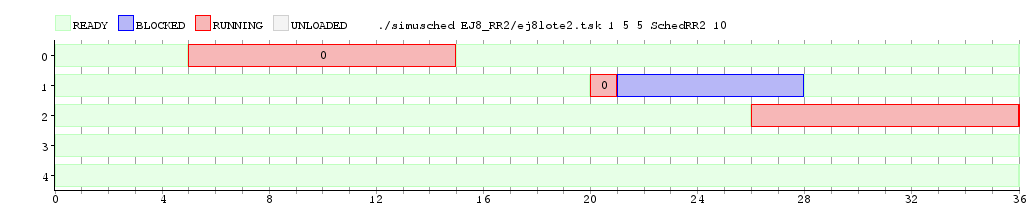
\includegraphics[width=450pt]{./EJ8_RR2/dif2corerr2.png}
	{$Lote 2$ - Round Robin 2 - 1 core - Quantum = 10 - cambio de contexto = 5}	
 \end{center}
 
 Viendose nuevamente, la igualdad que mencionamos. Hemos podido ver a su vez, que la única
 forma en la que los resultados sean distintos con el mismo lote seria modificando o la
 cantidad de $quantum$ o la unidad de cambio de contexto entre uno y otro.\\
 
 Aqui, un ejémplo para mayor precisión:\\
 
  \begin{center}
    	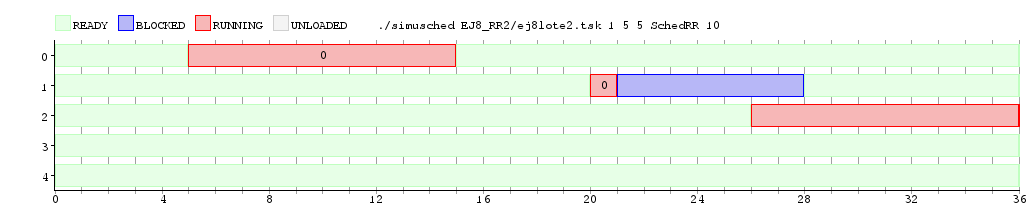
\includegraphics[width=450pt]{./EJ8_RR2/dif3corerr.png}
	{$Lote 2$ - Round Robin - 1 core - Quantum = 10 - cambio de contexto = 5}	
 \end{center}
 
 \begin{center}
    	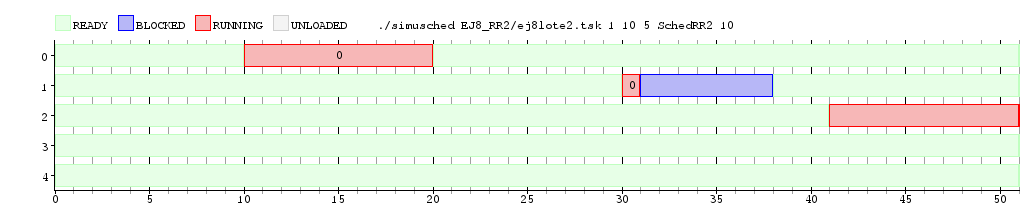
\includegraphics[width=450pt]{./EJ8_RR2/dif3corerr2.png}
	{$Lote 2$ - Round Robin 2 - 1 core - Quantum = 10 - cambio de contexto = 10}	
 \end{center}
 
 Concluimos entonces que, al trabajar con colas globales o no, utilizando un único núcleo y
 mismo lote quantum y cambio de contexto, ambos schedulers se comportan de la misma
 manera.\\
 
 Procedemos a demostrar la segunda conjetura:\\
 
 \textbf{Comportamiento menos eficiente en el RR2 con respecto al paralelismo, ya que al no permitir
migración de núcleos este lo pierde}\\

Para demostrar esta conjetura trabajamos con procesos que demanden mas uso del cpu como 
lo son las $taskCPU$\\

Un ejemplo de los lotes utilizados fue el siguiente:\\

\begin{verbatim}
                                     TaskCPU 40
                                     TaskCPU 15
                                     TaskCPU 50
                                     TaskCPU 30
                                     TaskCPU 50
\end{verbatim}

Obteniendo los siguientes datos relevantes:\\

\begin{center}
    	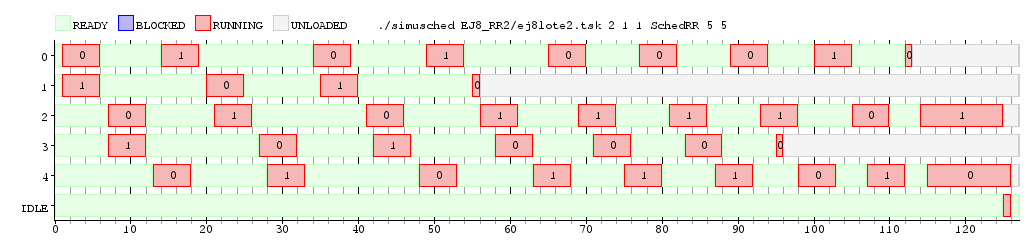
\includegraphics[width=450pt]{./EJ8_RR2/dif10corerr.png}
	{$Lote 3$ - Round Robin - 2 core - Quantum = 5 - cambio de contexto = 1}	
 \end{center}
 
 \begin{center}
    	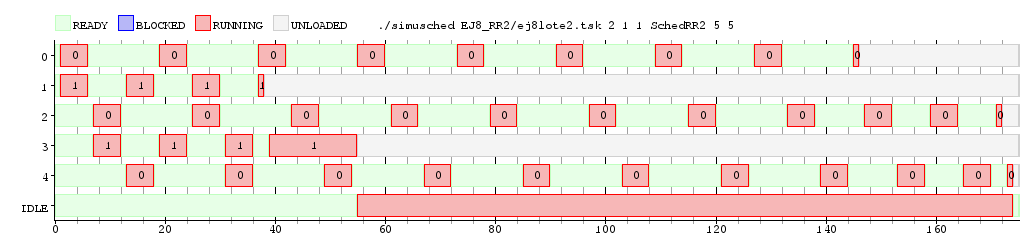
\includegraphics[width=450pt]{./EJ8_RR2/dif10corerr2.png}
	{$Lote 3$ - Round Robin 2 - 2 core - Quantum = 5 - cambio de contexto = 1}	
 \end{center}
 
 Se puede ver en estos diagramas como la implementación del Round Robin original trabaja
 mejor finalizando la ejecución de las tareas hasta 50 milisegundos antes.\\
 Esto se da por la falta de paralelismo de el RR2 ya que al ser asignados los procesos
 a cada core, cuando uno de los dos finaliza, este queda ocioso ya que no existe la
 posibilidad de migrar  procesos.\\
 
 Por ultimo, nuestra tercer y ultima conjetura:\\
 
 \textbf{Comportamiento mas eficiente en el RR2 con lotes de tareas que se bloquean un gran numero
de veces}

Para esta conjetura, trabajamos con lotes de tareas que utilicen el CPU y se bloqueen muchas
veces para poder demostrar la mejor performance del RR2.\\

A continuación un ejemplo, con el siguiente lote:

\begin{verbatim}
                                     TaskCPU 40
                                     TaskBatch 10  5
                                     TaskCPU 50
                                     TaskBatch 15 8
                                     TaskCPU 10

\end{verbatim}


   \begin{center}
    	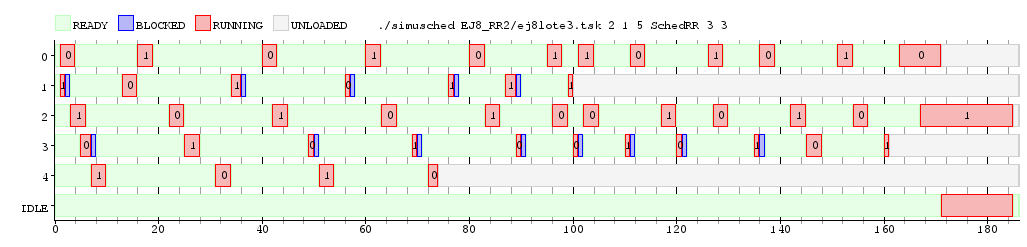
\includegraphics[width=450pt]{./EJ8_RR2/dif5corerr.png}
	{$Lote 3$ - Round Robin - 2 core - Quantum = 3 - cambio de contexto = 1}	
 \end{center}
 
 \begin{center}
    	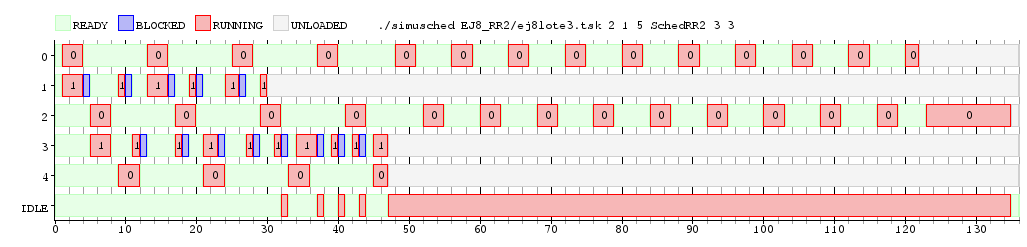
\includegraphics[width=450pt]{./EJ8_RR2/dif5corerr2.png}
	{$Lote 3$ - Round Robin 2 - 2 core - Quantum = 3 - cambio de contexto = 1}	
 \end{center}

 Se puede observar por los diagramas como el RR2 tiene una mejor performance en este estilo
 de lotes llegando a finalizar las ejecuciones hasta 50 milisegundos antes que el Round-Robin
 original.\\
 Como el Round-Robin original tiene pérdida de tiempo con el cambio de contexto y
 migración de tareas este empeora su performance en comparación al RR2 que no admite
 este tipo de migración es notorio la superioridad en relación a nuestra conjetura.\\
 
 Podemos concluir luego de estas demostraciones que, el Round-Robin original es ampliamente
 superior desde el punto de vista de la performance que se obtiene al trabajar con tareas
 que demanden mucho uso del CPU, mientras que el RR2 es ampliamente mejor cuando se utilicen
 tareas que se bloqueen por un tiempo considerable.\\
 


\newpage

\section{Parte 3: Evaluando los algoritmos de scheduling}


\subsection{Ejercicios}
\begin{itemize}
 
\item \textbf{Ejercicio 6}  Programar un tipo de tarea TaskBatch que reciba dos parametros: total cpu y
cant bloqueos. Una tarea de este tipo debera realizar cant bloqueos llamadas bloqueantes, en
momentos elegidos pseudoaleatoriamente. En cada tal ocasion, la tarea debera permanecer
bloqueada durante exactamente un (1) ciclo de reloj. El tiempo de CPU total que utilice una
tarea TaskBatch debera ser de total cpu ciclos de reloj (incluyendo el tiempo utilizado para
lanzar las llamadas bloqueantes; no ası el tiempo en que la tarea permanezca bloqueada).

\item \textbf{Ejercicio 7} Elegir al menos dos metricas diferentes, definirlas y explicar la semantica de
su definicion. Diseñar un lote de tareas TaskBatch, todas ellas con igual uso de CPU, pero
con diversas cantidades de bloqueos. Simular este lote utilizando el algoritmo SchedRR y una
variedad apropiada de valores de quantum. Mantener fijo en un (1) ciclo de reloj el costo de
cambio de contexto y dos (2) ciclos el de migracion. Deben variar la cantidad de nucleos de
procesamiento. Para cada una de las metricas elegidas, concluir cual es el valor optimo de
quantum a los efectos de dicha metrica.

\item \textbf{Ejercicio 8} Implemente un scheduler Round-Robin que no permita la migracion de procesos
entre nucleos (SchedRR2). La asignacion de CPU se debe realizar en el momento en que se produce la carga 
de un proceso (load). El nucleo correspondiente a un nuevo proceso sera aquel
con menor cantidad de procesos activos totales (RUNNING + BLOCKED + READY). Diseñe y realice un conjunto 
de experimentos que permita evaluar comparativamente las dos implementaciones de Round-Robin.

\item \textbf{Ejercicio 9} Diseñar y llevar a cabo un experimento que permita poner a prueba la ecuanimidad 
(fairness) del algoritmo SchedLottery implementado. Tener en cuenta que, debido
al factor pseudoaleatorio involucrado, cualquier corrida puntual podrıa ser arbitrariamente
injusta; sin embargo, si se repite un mismo experimento n veces y se observan los resultados acumulativos, 
tales anomalıas deberıan ir desapareciendo conforme n aumenta. En otras
palabras, interesa mostrar en base a evidencia empırica que el algoritmo implementado efectivamente tiende 
a ser totalmente ecuanime a medida que n tiende a infinito.

\item \textbf{Ejercicio 10} Los autores del artıculo sobre lottery scheduling alegan que la optimizacion de
compensation tickets es necesaria para compensar una posible falencia del algoritmo inicial-
mente propuesto en ciertos escenarios. Diseñar y llevar a cabo un experimento apropiado para
comprobar esta afirmacion (provocar un escenario donde se manifieste el problema, comparar
simulaciones ejecutadas con y sin compensation tickets y discutir los resultados obtenidos).

\end{itemize}
\subsection{Resultados y Conclusiones}

\subsubsection[Resolución Ejercicio 6]{Ejercicio 6}

\indent Al igual que con la tarea TaskConsola, mencionaremos nuestro implementación y acontinuación de la misma 
explicaremos ciertos puntos de la misma.\\
 \begin{verbatim}
                       void TaskBatch(int pid, vector<int> params) {
                            int total_cpu = params[0];
                            int cant_bloqueos = params[1];
                            srand(time(NULL));
                            vector<bool> uso = vector<bool>(total_cpu);
                            for(int i=0;i<(int)uso.size();i++) 
                               uso[i] = false;
	                       for(int i=0;i<cant_bloqueos;i++) {
                                   int j = rand()%(uso.size());
                                   if(!uso[j])
                                      uso[j] = true;
                                   else
                                      i--; 
                                   }
                            for(int i=0;i<(int)uso.size();i++) {
                                if( uso[i] )
                                    uso_IO(pid,1); 
                                else
                                    uso_CPU(pid, 1); 
                               }
                            }
 \end{verbatim}

 \indent Para este tipo de tarea, creamos un vector de tamaño igual a $total_cpu$ el cual tendra bool, ya sea true o false
 dependiendo del uso que se le de dentro de la tarea, ya sea uso\_IO o uso\_CPU. En caso de ser uso\_IO sera true, y sino false.\\
 Luego, utilizaremos un ciclo que ira desde 0 hasta el tamaño del vector y dependiendo el valor booleano, usará la funciones
 dadas por la catedra uso\_IO o uso\_CPU.\\
 
 \subsubsection[Resolución Ejercicio 7]{Ejercicio 7}
 Las métricas elegidas fueron:
\begin{itemize}
 \item \textbf{Turnaround}: Es el intervalo de tiempo desde que un proceso es cargado hasta que este finaliza su ejecución.
 \item \textbf{Waiting Time}: Es la suma de los intervalos de tiempo que un proceso estuvo en la cola de procesos $ready$.
\end{itemize}

\indent \indent Como las tareas TaskBatch se bloquean pseudoaleatoriamente, 
para obtener datos relevantes tomamos un promedio de las mediciones.\\
\indent A la hora de encarar la experimentación, lo que realizamos fue simular corridas con 
varios quantum para poder obtener una aproximación del efecto del $quantum$ en la ejecución del lote de tareas. 

\indent De esta aproximación, se confeccionaron gráficos de turnaround time en función del quantum, 
referente al estudio con 2 y 3 núcleos, los cuales se proveerán a continuación:\\

\indent Luego de realizar mediciones con distintos $quantum$, tomamos la decisión de trabajar con los mismos $quantum$ para cada nucleo
al trabajar con más de 1 core. (Se muestra acontinuación un gráfico para demostrar que no era una decisión acertada trabajar
con disversos $quantum$ para cada core).

\begin{center}
    	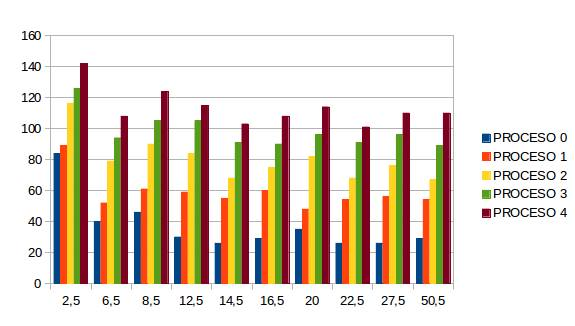
\includegraphics[width=1\textwidth]{./EJ7/turnarounddistquan.png}
	{Turnaround - 2 core - Prueba Quantum distintos por Core}\\
	{$Eje X = Quantum; $\\$ Eje Y = Tiempo$}\\
 \end{center}

\indent Al realizar, este gráfico y varias mediciones con distintos $quantum$ por core, nos dimos cuenta que no terminaban
siendo mediciones rigurosas, ya que una tarea podia estar corriendo con distintos tiempos por la migracion de procesos por core.\\
\indent Por ende, optamos por realizar mediciones con igualdad de $quantum$ por core para obtener la mejor performance posible.\\
 
 \indent Por consiguiente, al trabajar con las nuevas mediciones, conjeturamos las siguientes hipótesis:
 
 \begin{itemize}
  \item Con 2 nucleos las mediciones de tiempo tienden a estabilizarse a partir de un $quantum$ igual a 9.
  \item Con 3 nucleos las mediciones de tiempo tienden a estabilizarse a partir de un $quantum$ igual a 11.
 \end{itemize}
 \begin{center}
 \textbf{Turnaround Time} 
  \end{center}

 \begin{center}
 \textbf{2 Core}
 \end{center}
  A continuación se muestran los Diagramas de Gantt más relevantes:
  
  \begin{center}
    	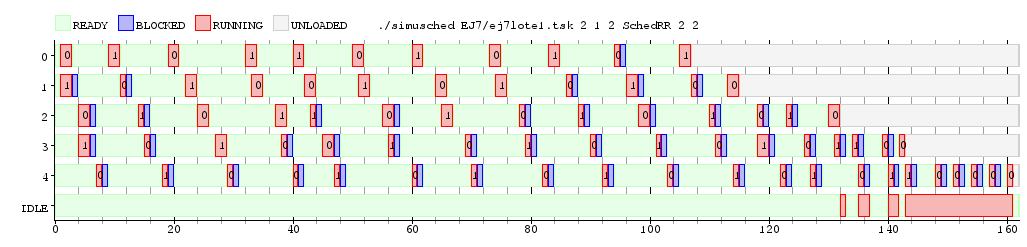
\includegraphics[width=450pt]{./EJ7/ej7tour2core1quan.png}
	{$Lote 1$ - Turnaround - 2 core - Quantum igual a 2}	
 \end{center}

   \begin{center}
    	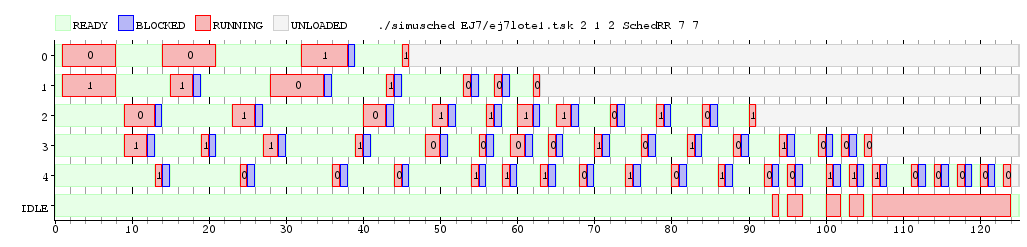
\includegraphics[width=450pt]{./EJ7/ej7tour2core3quan.png}
	{$Lote 1$ - Turnaround - 2 core - Quantum igual a 7}	
 \end{center}
 
 
 \indent La performance empieza a mejorar a medida que el $quantum$ aumenta.
 
   \begin{center}
    	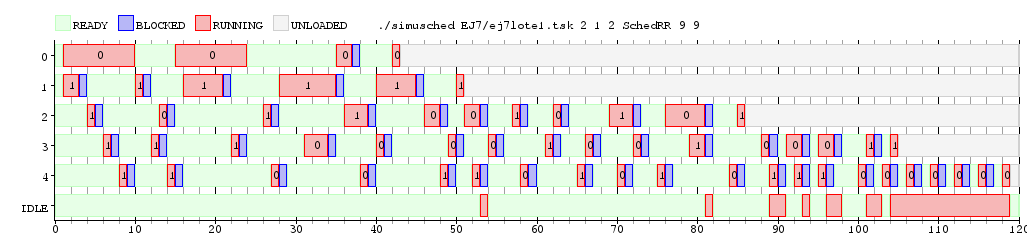
\includegraphics[width=450pt]{./EJ7/ej7tour2core4quan.png}
	{$Lote 1$ - Turnaround - 2 core - Quantum igual a 9}	
 \end{center}

  
   \indent La performance sigue mejorando,a partir de este valor, el desempeño comienza a estabilizarse, como muestran los siguiente dos gráficos. 
   Las pequeñas diferencias en los valores responden a la pseudoaleatoridad de las tareas TaskBatch.\\
  
   \begin{center}
    	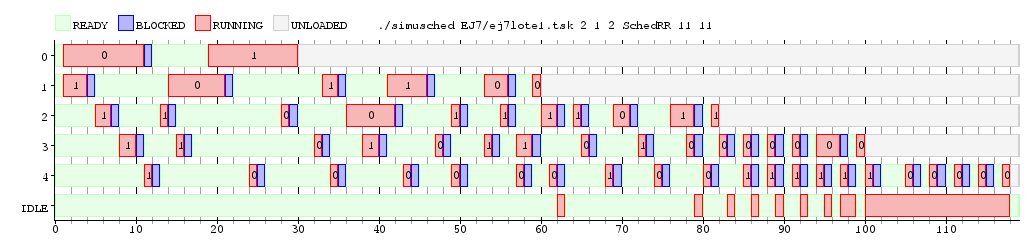
\includegraphics[width=450pt]{./EJ7/ej7tour2core5quan.png}
	{$Lote 1$ - Turnaround - 2 core - Quantum igual a 11}	
 \end{center}
 

    \begin{center}
    	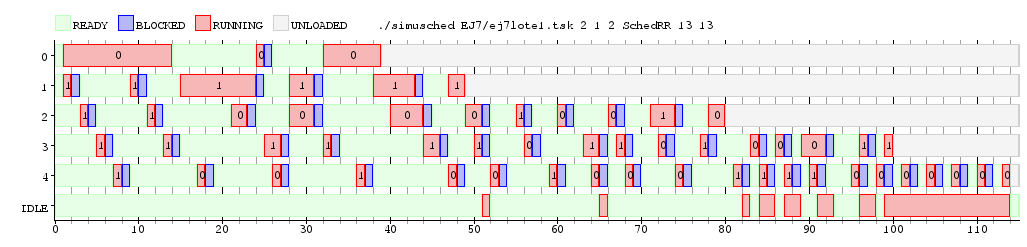
\includegraphics[width=450pt]{./EJ7/ej7tour2core8quan.png}
	{$Lote 1$ - Turnaround - 2 core - Quantum igual a 13}	
 \end{center}

 \indent Como mencionamos, las mediciones tienden a estabilizarse con un $quantum$ igual a 9, pero la mejor performance
 obtenida es con un $quantum$ igual a 13, teniendo en cuenta la pseudoaleatoridad del tipo de tarea utilizada.
 \indent Se puede observar en la primer figura que a pesar de trabajar con 2 cores, al tener un quantum bajo (igual a 2) 
 el costo es alto.\\
  
  
 \begin{center}
    	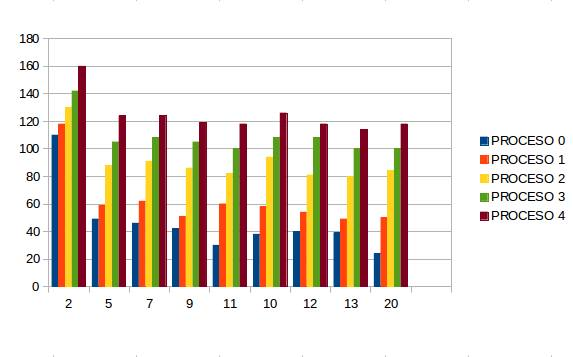
\includegraphics[width=1\textwidth]{./EJ7/tour2core.png}
	{Turnaround - 2 core}	\\
	{$Eje X = Quantum$\\$ Eje Y = Tiempo$}\\
 \end{center} 
 
 \begin{center}
  \textbf{Waiting Time}
 \end{center}

  \begin{center}
    	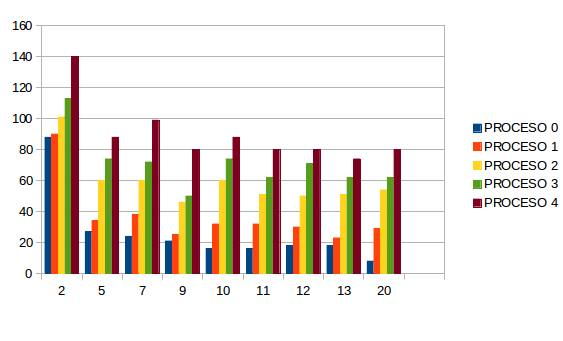
\includegraphics[width=1\textwidth]{./EJ7/waiting2core.jpg}
	{Waiting Time - 2 core}	\\
	{$Eje X = Quantum$\\$Eje Y = Tiempo$}\\
 \end{center} 
 
 \indent Con este tipo de metrica, se comienza a estabilizar a partir del $quantum$ igual a 5, obteniendo su mejor
 performance con el $quantum$ igual a 13.\\
 
   \begin{center}
   \textbf{3 Core}
   \end{center}
   \indent A continuación, al igual que con 2 cores, mostraremos los Diagramas de Gantt mas relevantes:
   
   \begin{center}
    	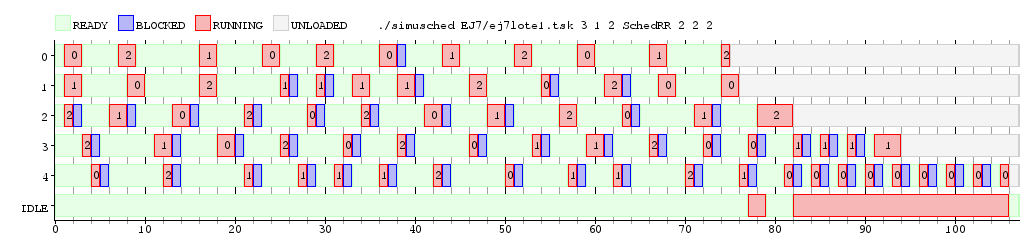
\includegraphics[width=450pt]{./EJ7/ej7tour3core1quan.png}
	{$Lote 1$ - Turnaround - 3 core - Quantum igual a 2}	
 \end{center}

 \indent Se observa que al tener otro core mas,a diferencia de con 2, a pesar de estar con un $quantum$ bajo,
 la performance mejora bastante.\\ 
 
   \begin{center}
    	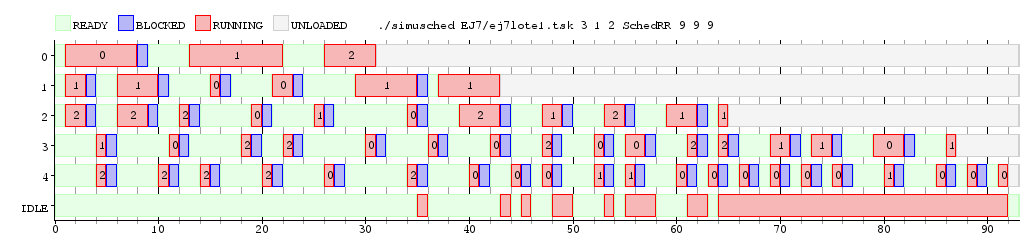
\includegraphics[width=450pt]{./EJ7/ej7tour3core4quan.png}
	{$Lote 1$ - Turnaround - 3 core - Quantum igual a 9}	
 \end{center}
 
 
 \indent La performance empieza a mejorar a medida que el $quantum$ aumenta.
 
   \begin{center}
    	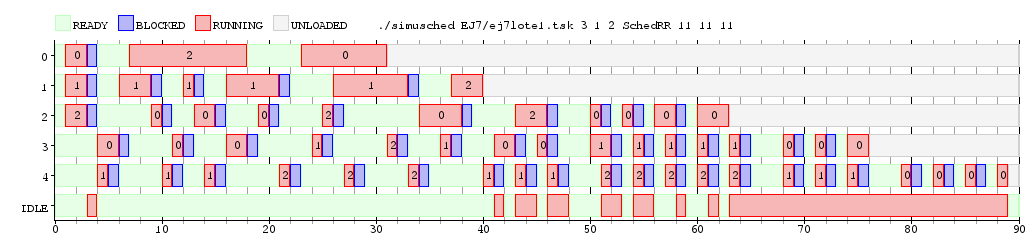
\includegraphics[width=450pt]{./EJ7/ej7tour3core5quan.png}
	{$Lote 1$ - Turnaround - 3 core - Quantum igual a 11}	
 \end{center}
  
   \begin{center}
    	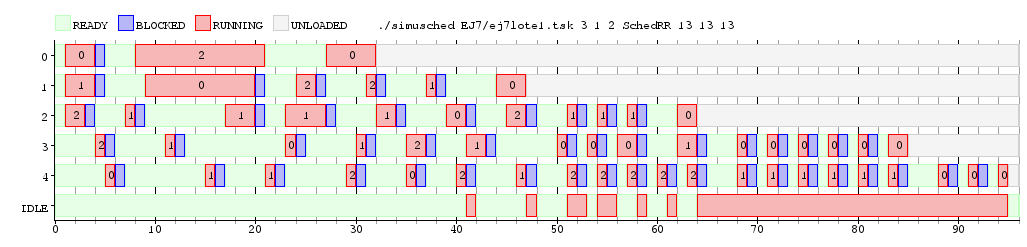
\includegraphics[width=450pt]{./EJ7/ej7tour7core6quan.png}
	{$Lote 1$ - Turnaround - 3 core - Quantum igual a 13}	
 \end{center}
 
 \begin{center}
    	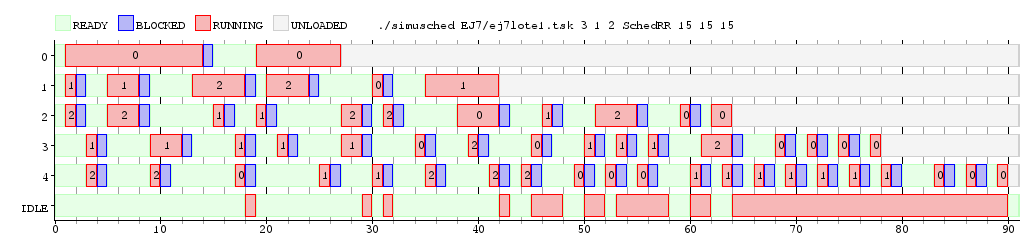
\includegraphics[width=450pt]{./EJ7/ej7tour8core6quan.png}
	{$Lote 1$ - Turnaround - 3 core - Quantum igual a 15}	
 \end{center}
 
 \indent A diferencia que en nuestra hipótesis conjeturada para con dos cores, con un $quantum$ igual a 11 se obtiene la mejor
 performance, pero teniendo en cuenta la pseudoaleatoridad del tipo de tarea con la que se trabajo, a partir del $quantum$ igual
 a 9 ya se estabiliza notoriamente.\\
   
    \begin{center}
    	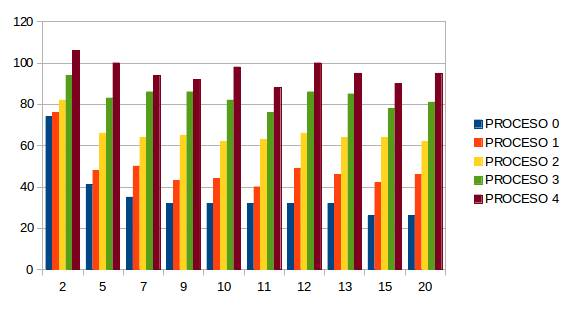
\includegraphics[width=1\textwidth]{./EJ7/tour3core.png}
	{Turnaround - 3 core}\\
	{$Eje X = Quantum $\\$ Eje Y = Tiempo$}\\
 \end{center} 
  
   \begin{center}
  \textbf{Waiting Time}
 \end{center}

  \begin{center}
    	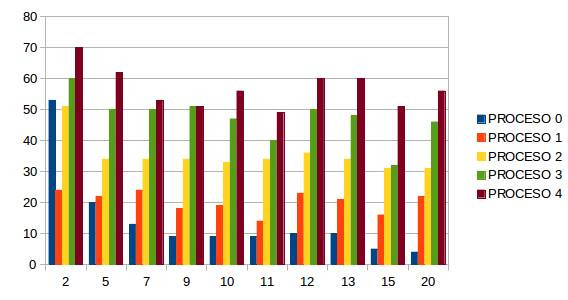
\includegraphics[width=1\textwidth]{./EJ7/waintin3core.jpg}
	{Waiting Time - 3 core}	\\
	{$Eje X = Quantum $\\$Eje Y = Tiempo$}\\
 \end{center} 
 
   \indent Con este tipo de metrica,se obteniene a diferencia de con Turnaround  su mejor
   performance con el $quantum$ igual a 15.\\
  
 \begin{center}
  \textbf{Conclusiones}
 \end{center}


\indent \indent La diferencia entre los valores de quantum entre los casos se puede atribuir a que cada vez que 
agregamos un núcleo aumentamos la posibilidad de una migración de la tareas.\\
\indent \indent En todos lo casos se observa la influencia negativa que proviene de elegir un quantum con valores pequeños.\\
\indent \indent Agregar núcleos de procesamiento mejora significativamente la performance de acuerdo a la métricas con las que
trabajamos, al permitir más procesamiento en pararelo y disminuyendo los waiting time de las tareas.\\
\indent \indent  Fijada una cantidad de núcleos, aumentar el valor del quantum también mejora la performance, 
especialmente los tiempos referidos a las tareas que menos cantidad de bloqueos tienen. 
Igualmente, a partir de cierto valor de quantum, las mejoras en la performance dejan de ser muy significativas. 
Esto se produce a que las tareas con mas cantidad de bloqueos en algun momento dejan de consumir todo
su quantum si seguimos aumentando el valor. 
 
 
 
\subsubsection[Resolución Ejercicio 8]{Ejercicio 8}
\indent \indent La idea central de esta version de Round-Robin es que no permita migración entre núcleos y esto se basa en utilizar una cola FIFO por cada núcleo, donde se encolarán aquellas tareas a las que se asignó el core correspondiente. \\ 
\indent Para implementar este algoritmo, el Round-Robin 2, utilizamos varias estructuras. Estas son:\\
\begin{itemize}
\item Los vectores $quantum$ y $quantumActual$, que cumplen la misma función que en nuestra implementación de Round-Robin.\\
\item El vector de colas $colas$, donde en la posición $i$ se encontrará la cola de tareas correspondiente a ese núcleo de procesamiento.\\
\item El diccionario $bloqueados$, donde mantenemos aquellas tareas que se bloquearon con su número de core correspondiente y que nos permitirá, cuando la tarea se desbloquee, reubicarla en la cola del core que le corresponde.\\ 
\item El vector de enteros $cantidad$, cuya única función será tener en la posición $i$ la cantidad de tareas bloqueadas, activas o en estado ready que están asignadas al core $i$ y que nos servirá para determinar a qué núcleo se asignará una tarea al momento de cargarla.\\
\end{itemize}

\indent \indent Cuando se carga una tarea, se chequea cuál es el core que menor cantidad de procesos activos totales tiene asignados(haciendo uso de la posición respectiva del vector $cantidad$). Una vez que se obtiene dicho núcleo, se agrega la tarea a la cola de tareas correspondiente al core y se actualiza la cantidad de tareas activas para ese núcleo sumándole uno.\\
\indent \indent Al bloquearse una tarea, se define una entrada en el diccionario $bloqueados$ con el pid y el núcleo correspondiente. De esta manera, al desbloquearse, obtenemos el core en el que debe correr, eliminamos la entrada del diccionario y encolamos nuevamente el pid a la cola del núcleo en cuestión. De esta manera resolvemos parcialmente el problema de no permitir la migración entre cores.\\
\indent \indent Finalmente, cuando una tarea termina, se actualiza la cantidad correspondiente al núcleo restándole uno. Solamente a la hora de cargar la tarea y cuando una tarea termina se modifica dicha variable. De esta manera, aunque una tarea se bloquee seguirá reflejada en la cantidad del núcleo, lo que nos permitirá seguir el criterio que nos pidieron en la consigna a la hora de asignarle un core a la tarea.\\

\indent \indent Como esta modificación de Round-Robin no permite migración entre cores, 
conjeturamos ciertos puntos:\\
\begin{itemize}
 \item Dados un mismo lote de tareas y una misma configuración del scheduler (tick de costo en cambio de contexto y quantum)
 un único núcleo de procesamiento,  ambos algoritmos deben comportarse de la misma manera. 
  \item Comportamiento más eficiente en el Round-Robin 2 en lotes de tareas que se bloquean una gran cantidad de veces, o  en configuraciones con $quantums$ pequeños. 
  Esto surge de que dichos escenarioshacen más proclive al Round-Robin a impulsar más cambios de contexto, 
  con la posible penalidad de darse un cambio de núcleo, algo que puede ser muy costoso.
  \item El Round Robin debería comportarse más eficientemente en situaciones en las cuales el Round-Robin 2 pierde la posibilidad de parelelismo. 
  Por ejemplo, varias tareas quedaron asignadas a un núcleo mientras los demás están libres. Generando que varios nucleos queden ociosamente bastante tiempo.
  
 \end{itemize}

 \indent A continuación, mostraremos los experimentos diseñados para demostrar y explicar un poco mejor lo conjeturado:
 
 \indent Arrancando con nuestra primer conjetura:
 
 \begin{center}
  \textbf{Dados un mismo lote de tareas y una misma configuración del scheduler con un único núcleo de procesamiento, 
 ambos algoritmos deben comportarse de la misma manera. }
 \end{center}

 
 \indent Trabajando con el siguiente lote:
 
 \begin{verbatim}
                                     TaskCPU 70
                                     TaskConsola 2 4 5
                                     TaskCPU 40
                                     TaskConsola 3 2 3
                                     TaskCPU 30
 \end{verbatim}

  \begin{center}
    	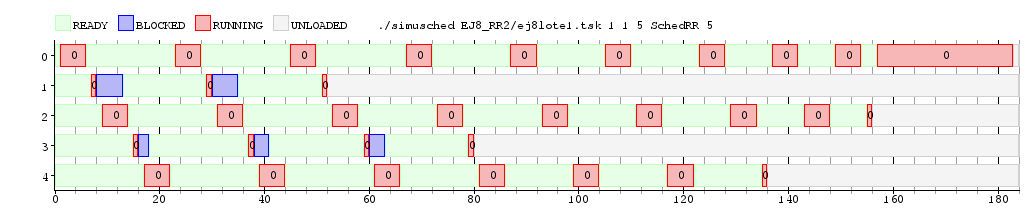
\includegraphics[width=450pt]{./EJ8_RR2/dif1corerr.png}
	{$Lote 1$ - Round Robin - 1 core - Quantum = 5 - cambio de contexto = 1}	
 \end{center}
 
 \begin{center}
    	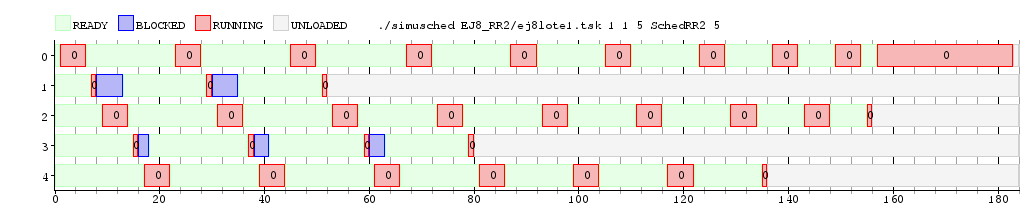
\includegraphics[width=450pt]{./EJ8_RR2/dif1corerr2.png}
	{$Lote 1$ - Round Robin 2 - 1 core - Quantum = 5 - cambio de contexto = 1}	
 \end{center}
 
 \indent Se ve a simple vista, la igualdad entre ambos con este tipo de lote.\\
 
 \indent Ahora, con un lote distinto:
 
 \begin{verbatim}
                                     TaskCPU 70
                                     TaskConsola 5 6 7
                                     TaskCPU 40
                                     TaskConsola 10 9 8
                                     TaskCPU 30
 \end{verbatim}
 
   \begin{center}
    	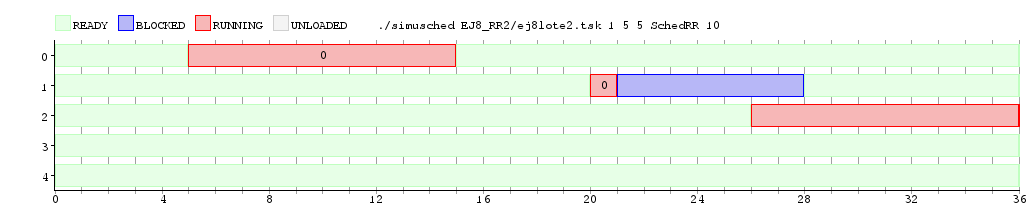
\includegraphics[width=450pt]{./EJ8_RR2/dif2corerr.png}
	{$Lote 2$ - Round Robin - 1 core - Quantum = 10 - cambio de contexto = 5}	
 \end{center}
 
 \begin{center}
    	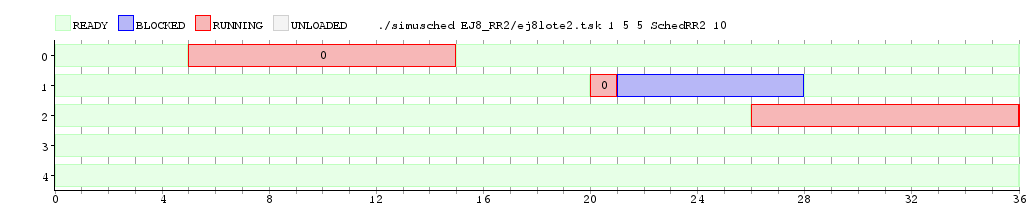
\includegraphics[width=450pt]{./EJ8_RR2/dif2corerr2.png}
	{$Lote 2$ - Round Robin 2 - 1 core - Quantum = 10 - cambio de contexto = 5}	
 \end{center}
 
 \indent Nuevamente, observamos la misma igualdad entre ambos. De la unica manera en la cual se podria producir un cambio
 entre ambos Diagramas es alterando el cambio de contexto para uno y no para el otro.
 
 \begin{center}
    	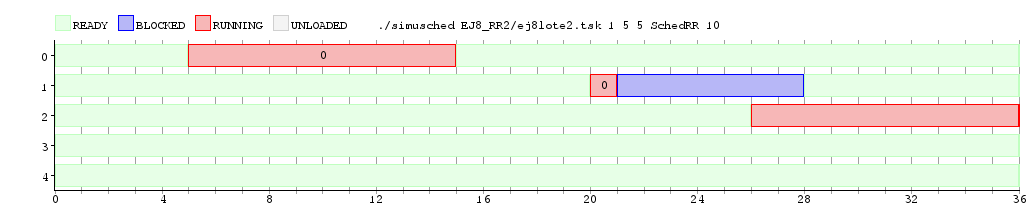
\includegraphics[width=450pt]{./EJ8_RR2/dif3corerr.png}
	{$Lote 2$ - Round Robin - 1 core - Quantum = 10 - cambio de contexto = 5}	
 \end{center}
 
 \begin{center}
    	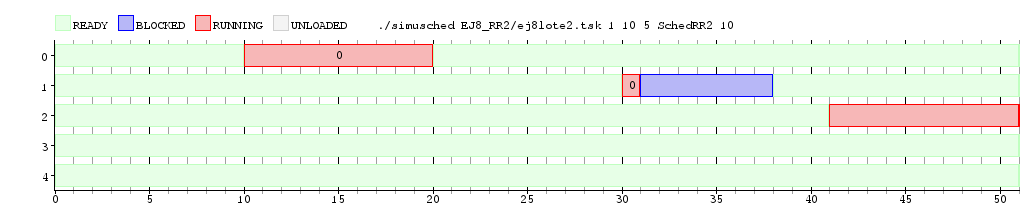
\includegraphics[width=450pt]{./EJ8_RR2/dif3corerr2.png}
	{$Lote 2$ - Round Robin 2 - 1 core - Quantum = 10 - cambio de contexto = 10}	
 \end{center}
 
  \indent Aqui se ve las diferencias como lo mencionamos, por ende, podemos concluir que como el Round Robin 2 solo fue modificado 
  para tener colas independientes para cada nucleo, al trabajar con 1 solo core, no se veran diferencias.\\

  \indent Continuamos con la siguiente conjetura realizada:
  
  \begin{center}
   \textbf{Comportamiento más eficiente en el Round-Robin 2 en lotes de tareas que se bloquean una gran cantidad de veces, 
   o  en configuraciones con $quantums$ pequeños.}
  \end{center}
  
  \indent Arrancaremos mostrando casos con cambios de contexto y quantum pequeños:
  
   \begin{center}
    	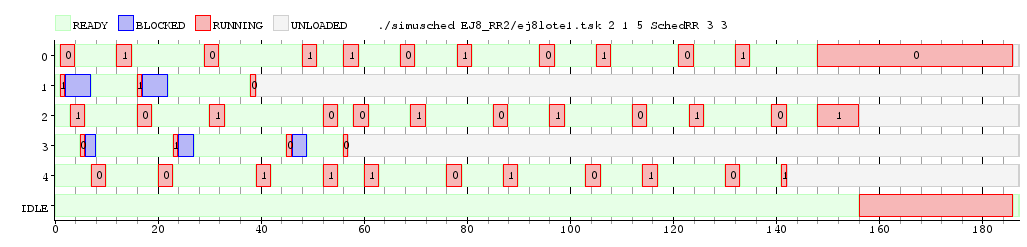
\includegraphics[width=450pt]{./EJ8_RR2/dif4corerr.png}
	{$Lote 1$ - Round Robin - 2 core - Quantum = 3 - cambio de contexto = 1}	
 \end{center}
 
 \begin{center}
    	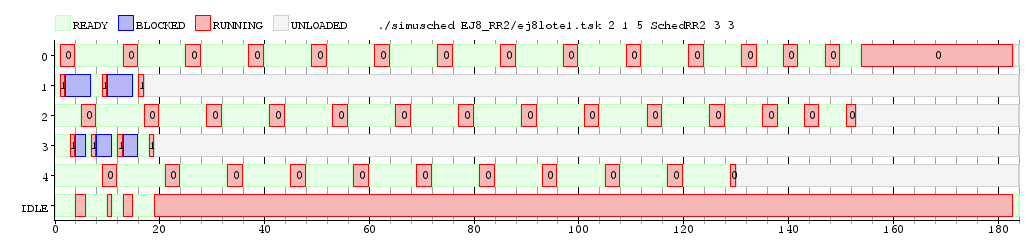
\includegraphics[width=450pt]{./EJ8_RR2/dif4corerr2.png}
	{$Lote 1$ - Round Robin 2 - 2 core - Quantum = 3 - cambio de contexto = 1}	
 \end{center}
 
 
\indent Se puede observar, una mejoria leve del Round Robin 2. Con la modificación realizada en el Round Robin 2,
no habria ninguna modificacion en caso de aumentar o disminuir el cambio de migracion ya que este no lo permite.\\

\indent Ahora, si trabajamos con tareas que utilicen el CPU y se bloqueen mucho mas podremos notar la mejor performance
de este nuevo scheduler.\\

\begin{verbatim}
                                     TaskCPU 40
                                     TaskBatch 10  5
                                     TaskCPU 50
                                     TaskBatch 15 8
                                     TaskCPU 10

\end{verbatim}


   \begin{center}
    	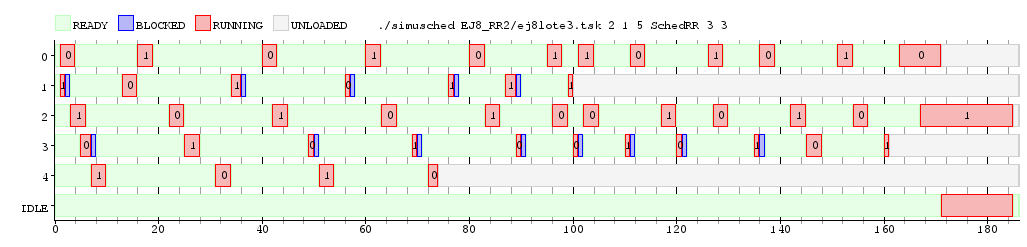
\includegraphics[width=450pt]{./EJ8_RR2/dif5corerr.png}
	{$Lote 3$ - Round Robin - 2 core - Quantum = 3 - cambio de contexto = 1}	
 \end{center}
 
 \begin{center}
    	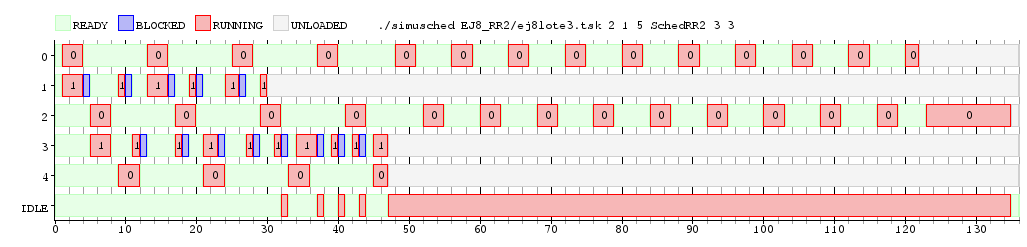
\includegraphics[width=450pt]{./EJ8_RR2/dif5corerr2.png}
	{$Lote 3$ - Round Robin 2 - 2 core - Quantum = 3 - cambio de contexto = 1}	
 \end{center}

 \indent Se ve a simple vista, como el RR2 es mucho mejor, y termina aprox 50 milisegundos antes.\\
 Como mencionamos anteriormente, si el cambio de migracion se alterase no tendria incidencia para este RR2 ya que 
 no admite migracion de tareas, mientras que el anterior scheduler si, pudiendo empeorar a su vez su performance en caso
 de que el coso fuese mayor.\\
 
 \indent Por consiguiente, podemos afirmar, que nuestro RR2 sera notablemente mejor con tareas que utilicen el CPU y se bloqueen
 bastante tiempo.\\
 
 \indent Por ulimto, demostraremos nuestra ultima conjetura: 
 
  \begin{center}
   \textbf{El Round Robin debería comportarse más eficientemente en situaciones en
   las cuales el Round-Robin 2 pierde la posibilidad de parelelismo.}
  \end{center}
  
  \indent Para probar esta conjetura, utilizamos tareas que demanden mas al CPU como $TaskCPU$.\\
  
\begin{verbatim}
                                     TaskCPU 40
                                     TaskCPU 15
                                     TaskCPU 50
                                     TaskCPU 30
                                     TaskCPU 50
\end{verbatim}

\begin{center}
    	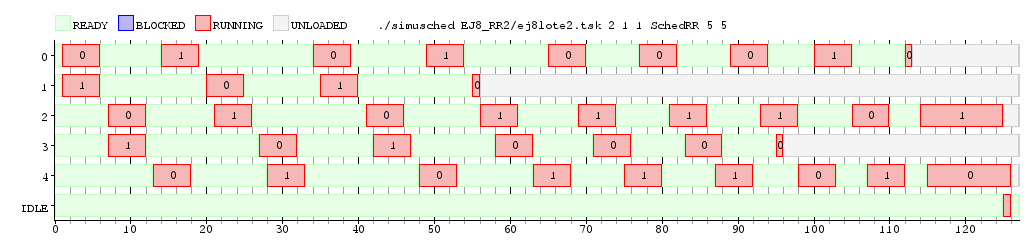
\includegraphics[width=450pt]{./EJ8_RR2/dif10corerr.png}
	{$Lote 3$ - Round Robin - 2 core - Quantum = 5 - cambio de contexto = 1}	
 \end{center}
 
 \begin{center}
    	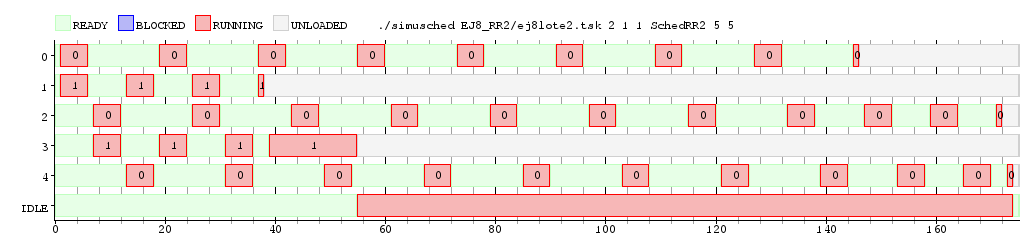
\includegraphics[width=450pt]{./EJ8_RR2/dif10corerr2.png}
	{$Lote 3$ - Round Robin 2 - 2 core - Quantum = 5 - cambio de contexto = 1}	
 \end{center}

 \indent Es notorio en estos gráficos cómo el Round-Robin, responde mejor que el Round-Robin 2. 
 Esto es porque puede trabajar con procesamiento en paralelo, mientras que el Round-Robin 2 no, 
 porque las 3 tareas quedaron asignadas a un core (el numero 0), aunque haya un core ocioso por un largo tiempo.\\
 En este caso, pagando el costo de migración se obtiene una mejor performance.\\

\indent Con estos experimentos realizados logramos observar los comportamientos que habíamos conjeturado concluyendo que son
ciertos. 

\indent Por ende, podemos concluir que el Round-Robin 2 responde de manera positiva para lotes con tareas de gran cantidad de bloqueos
y de manera negativa al no poder paralelizar ciertos procesos.\\
  
\subsubsection[Resolución Ejercicio 9]{Ejercicio 9}

\subsubsection[Resolución Ejercicio 10]{Ejercicio 10}

\indent Hemos encontrado, luego de varios experimentos, que este tipo de scheduler presenta graves problemas cuando 
se tienen varias tareas con mismo deadline.\\
Al no presentar ningun tipo de especificación, este scheduler, al no saber cuanto durará la tarea ejecuta cualquiera sin
darle prioridad al orden de los deadline dado en el lote de tarea.\\
A continuación, expondremos un caso practico donde se puede ver como impacta dentro del desempeño del scheduler el orden en el que son
cargadas las tareas pero la falta de informacion del scheduler imposibilita la posibilidad de cumplir la propiedad
de carga respetando los deadline dados.\\

Uno de los lotes propuestos, fue el siguiente:\\
\\\\\\\\
\begin{verbatim}
                                         $5:
                                         TaskCPU 40
                                         $25:
                                         TaskConsola 2 5 8
                                         $25:
                                         TaskCPU 100
                                         $25:
                                         TaskConsola 1 1 5

\end{verbatim}

Donde el resultado que obtuvimos fue el siguiente:\\

 \begin{center}
    	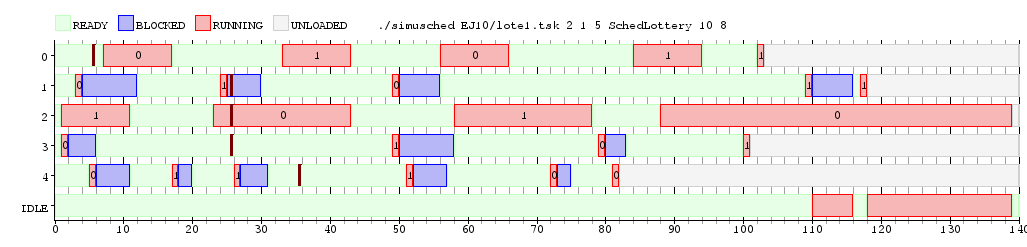
\includegraphics[width=450pt]{./ej10p7con.png}
	{$Lote 2$ - Lottery - 2 core}	
 \end{center}

\indent Como se puede observar, tanto el proceso 2 como 3 y 4 presentan el mismo deadline y terminan corriendo
fuera del orden acordado a pesar de estar trabajando con varios cores a la ves.\\

\indent Tambien, desarrollamos experimentos para los casos en que los deadline no sean los mismos, y obtuvimos
resultados similares.\\
Uno de los lotes fue el siguiente:

\begin{verbatim}
                                         $5:
                                         TaskCPU 40
                                         $25:
                                         TaskConsola 2 5 8
                                         $30:
                                         TaskCPU 100
                                         $35:
                                         TaskConsola 1 1 5

\end{verbatim}

Donde el resultado fue:\\

 \begin{center}
    	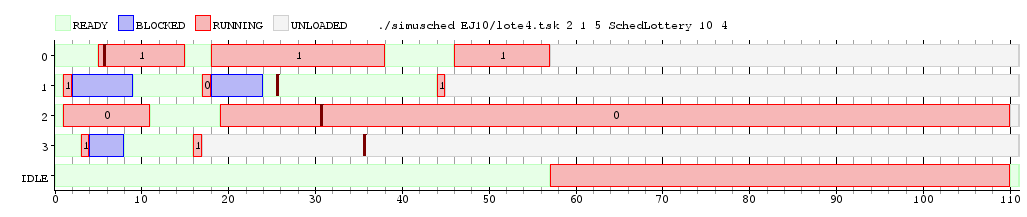
\includegraphics[width=450pt]{./ej10p12con.png}
	{$Lote 4$ - Lottery - 2 core}	
 \end{center}

 \indent Como vemos, a pesar de tener distintos valores de deadline no se respeta el orden en este scheduler.\\

\newpage


%%%%%%%%%%%%%%%%%%%%%%%%%%%%%%%%%%%%%%%%%%%%%%%%%%%%%%%%%%%%%%%%%%%%%%%%%%%%%%%
%% Conclusión                                                                %%
%%%%%%%%%%%%%%%%%%%%%%%%%%%%%%%%%%%%%%%%%%%%%%%%%%%%%%%%%%%%%%%%%%%%%%%%%%%%%%%

\newpage
\section{Bibliografía}

\begin{itemize}
 \item Cátedra de Sistemas Operativos - Clases teóricas y prácticas (2º Cuatrimestre 2014)
 \item Facultad de Ingenieria Uruguay \\
 $(https://eva.fing.edu.uy/pluginfile.php/75120/mod\_resource/content/1/6-SO-Teo-Planificacion.pdf)$
 \item Operating Systems Concepts, Abraham Silberschatz \& Peter B. Galvin
\end{itemize}

\end{document}
